% 1998 年全国卷理科第 23 题：斜三棱柱 ABC-A_1B_1C_1
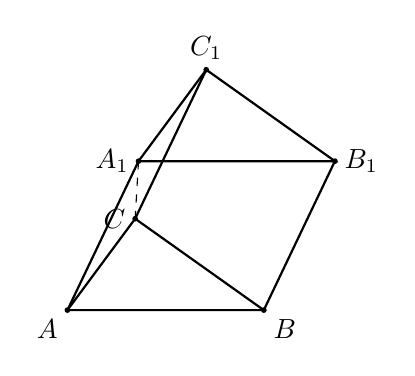
\begin{tikzpicture}[>=stealth, scale=0.86]
  \coordinate (A) at (0,0);
  \coordinate (B) at (2.9,0);
  \coordinate (C) at (1.0,1.35);
  \coordinate (A1) at (1.05,2.2);
  \coordinate (B1) at (3.95,2.2);
  \coordinate (C1) at (2.05,3.55);
  \draw[thick] (A)--(B)--(C)--cycle;
  \draw[thick] (A1)--(B1)--(C1)--cycle;
  \draw[thick] (A)--(A1) (B)--(B1) (C)--(C1);
  \draw[dashed] (A1)--(C) (A)--(C);
  \fill (A) circle (1.2pt) node[below left] {$A$};
  \fill (B) circle (1.2pt) node[below right] {$B$};
  \fill (C) circle (1.2pt) node[left] {$C$};
  \fill (A1) circle (1.2pt) node[left] {$A_1$};
  \fill (B1) circle (1.2pt) node[right] {$B_1$};
  \fill (C1) circle (1.2pt) node[above] {$C_1$};
\end{tikzpicture}
